\section{Analytical dispersion relations}
\subsection{Eigenvalue problem}
In a two dimensional $(x, z)$ plan, we consider the system of compressible adiabatic equations written under conservative form:
\[
\begin{array}{lcl}
\displaystyle \frac{{\rm D} \rho u}{{\rm D} t}&=&\displaystyle -\frac{\partial p}{\partial x}\\[4mm]
\displaystyle \frac{{\rm D} \rho w}{{\rm D} t}&=&\displaystyle -\frac{\partial p}{\partial z}-\rho g\\[4mm]
\displaystyle \frac{{\rm D}\rho}{{\rm D}t}&=&\displaystyle -\rho \nabla \cdot u\\[4mm]
\displaystyle \frac{{\rm D}p}{{\rm D}t}&=&\displaystyle c_s^2\frac{{\rm D}\rho}{{\rm D}t}=-c_s^2\rho \nabla \cdot u,
\end{array}
\]
where $(u, w$) are the horizontal and vertical velocity components, $\rho$ the density and $p$ the pressure. The speed of sound $c_s$ is assumed to be a constant.\\
These equations are linearized around a state at rest $(u(x,z,t)=u_0+u'(x,z,t), w(x,z,t)=w_0+w'(x,z,t), u_0 = w_0 = 0)$ and in hydrostatic equilibrium.
We decompose pressure and density fields around horizontally homogeneous background fields:
\[
p(x,z,t)=\overline{p}(z)+p'(x,z,t),\quad \rho(x,z,t)=\rho_0(z)+\rho'(x,z,t),
\]
where the backgroud fields are in hydrostatic balance:
\[
\frac{{\rm d} \overline{p}(z)}{{\rm d} z}=-\rho_0(z)g.
\]
Introducing the Brunt-V\"ais\"al\"a frequency
\[
N^2=-\frac{g}{\rho_0(z)}\frac{{\rm d} \rho_0(z)}{{\rm d} z}-\frac{g^2}{c_s^2},
\]
the vertical derivative of the background density field is given by
\[
\frac{{\rm d} \rho_0(z)}{{\rm d} z}=\rho_0(z)\left(
-\frac{N^2}{g}-\frac{g}{c_s^2}
\right).
\]
Or by defining a scale depth $D(z)$ by
\[
\frac{1}{D(z)}=\frac{N^2(z)}{g}+\frac{g}{c_s^2},
\]
\begin{equation}
\frac{{\rm d} \rho_0(z)}{{\rm d} z}=-\frac{\rho_0(z)}{D(z)}.
\label{eqrhodz}
\end{equation}
The system satisfied by the pertubations can be expressed as (dropping the ')
\begin{align*}
\frac{\partial \rho_0 u}{\partial t}&=-\frac{\partial p}{\partial x}\\
\frac{\partial \rho_0 w}{\partial t}&=-\left(\frac{\partial p}{\partial z}+g\rho\right)\\
\frac{\partial \rho}{\partial t}&=-\left(\frac{\partial \rho_0 u}{\partial x}+\frac{\partial \rho_0 w}{\partial z}\right)\\
\frac{\partial p}{\partial t}&=-c_s^2\left(
\displaystyle \frac{\partial \rho_0 u}{\partial x}+\frac{\partial \rho_0 w}{\partial z}
\right)+\left(
-\frac{c_s^2}{D(z)}+g
\right)\rho_0w,
\end{align*}
where we have made use of Eq. (\ref{eqrhodz}) to insert $\rho_0(z)$ inside the divergence terms. This system is linear in the variables $\rho_0u, \rho_0w, \rho, p$.\\
The system is complemented by the following bottom and surface boundary conditions: $w(-H)=0, \displaystyle \frac{\partial \eta}{\partial t}=w(0)$, where $\eta(x,t)$ is the surface elevation. In term of pressure, the linearized surface boundary condition writes $\displaystyle \frac{\partial p}{\partial t}=\rho_0(0)gw(0)$.
\\
Looking for plane waves solution of the form
\[
\left(
\begin{array}{c}
\rho_0 u\\
\rho_0 w\\
\rho\\
p
\end{array}
\right)
=
\left(
\begin{array}{c}
\widetilde{U}(z)\\
\widetilde{W}(z)\\
R(z)\\
P(z)
\end{array}
\right)
e^{i(k_xx-\sigma t)},
\]
we can obtain that $\widetilde{W}$ has to be solution of the following second order differential equation
\begin{equation}
\widetilde{W}''(z)+\frac{1}{D(z)}\widetilde{W}'(z)
+
\left(
k_x^2\frac{N^2-\sigma^2}{\sigma^2}+\frac{\sigma^2}{c_s^2}
-\frac{D'(z)}{D^2(z)}
\right)
\widetilde{W}(z)=0
\label{eqwfirst}
\end{equation}
This system has been derived in Dukowicz in the case of constant Brunt-V\"ais\"al\"a frequency and in a vertically lagragian coordinate system.\\
The first order term in Eq. (\ref{eqwfirst}) can be removed by a change of variable, namely,
\[
\widetilde{W}(z)=e^{\int_{z}^0\frac{1}{2D(z_1)}{\rm d}z_1}F(z),
\]
to obtain
\begin{equation}
F''(z)
+\left(
k_x^2\frac{N^2-\sigma^2}{\sigma^2}
+
\frac{\sigma^2}{c_s^2}-\frac{1}{4D(z)^2}(1+2D'(z))
\right)
F(z)=0
\label{eqF}
\end{equation}
which corresponds to Eq. (28, 29) of Dukowicz (2013) in the general case of variable Brunt-V\"ais\"al\"a frequency.
\\
The polarization relations that link horizontal velocity and pressure pertubations to vertical velocity perturbations are given by\footnote{We do not consider the special case of Lamb waves for which $\sigma^2=c_s^2k_x^2$.}
\[
\begin{array}{rcl}
\widetilde{U}(z)&=&\displaystyle  -ik_x\frac{(c_s^2-gD(z))\widetilde{W}(z)+c_s^2D(z)\widetilde{W}'(z)}{D(z)(\sigma^2-c_s^2k_x^2)}\\[4mm]
\rho(z)&=&\displaystyle -i\frac{k_x^2(c_s^2-gD(z))\widetilde{W}(z)+\sigma^2D(z)\widetilde{W}'(z)}{\sigma(\sigma^2-c_s^2k_x^2)D(z)}\\[4mm]
P(z)&=&\displaystyle -i\sigma\frac{(c_s^2-gD(z))\widetilde{W}(z)+c_s^2D(z)\widetilde{W}'(z)}{(\sigma^2-c_s^2k_x^2)D(z)}
\end{array}
\]
The linearized surface boundary condition $\displaystyle \frac{\partial p(z=0)}{\partial t}=g \rho_0(0)w(0)$ leads to
\[
-i\sigma P(0)=g \widetilde{W}(0)
\]
or
\[
\widetilde{W}'(0)+\left(
\frac{1}{D(0)}-\frac{gk_x^2}{\sigma^2}
\right)\widetilde{W}(0)=0
\]
or in term of the function $F$ as
\begin{equation}
F'(0)+\left(
\frac{1}{2D(0)}-\frac{gk_x^2}{\sigma^2}
\right)F(0)=0
\label{eqFbc}
\end{equation}
The bottom boundary condition $w(x,z=-H,t)=0$ imposes $F(-H)=0$. The general solution is thus obtained by solving the eigenvalue problem for the squarred frequency $\sigma^2$ composed of Eqs. (\ref{eqF}, \ref{eqFbc}) and the bottom boundary condition:
\[
\begin{array}{l}
\displaystyle
F''(z)
+\left(
k_x^2\frac{N^2-\sigma^2}{\sigma^2}
+
\frac{\sigma^2}{c_s^2}-\frac{1}{4D^2}(1+2D'(z))
\right)
F(z)=0\\[4mm]
\displaystyle
F'(0)+\left(
\frac{1}{2D(0)}-\frac{gk_x^2}{\sigma^2}
\right)F(0)=0\\[4mm]
\displaystyle
F(-H)=0
\end{array}
\]
%
%They are not valid when the frequency $\sigma$ is given by $\sigma^2=c_s^2k_x^2$. When $\sigma^2=c_s^2k_x^2$, $W(z)$ has to satisfy
%\[
%W'(z)=\frac{-c_s^2+gD}{c_s^2D}W(z)
%\]
%and thus due to the boundary condition $W(-H)=0$, $W(z)$ is identically zero and we get
%\[
%\begin{array}{rcl}
%P'(z)&=&\displaystyle -\frac{g}{c_s^2}P(z)\\[4mm]
%U(z)&=&\displaystyle \frac{k_x}{\sigma}P(z)\\[4mm]
%\rho(z)&=&\displaystyle \frac{P(z)}{c_s^2}
%\end{array}
%\]
%This corresponds to Lamb waves.
\subsubsection{The constant Brunt-V\"ais\"al\"a case}
When the Brunt-V\"ais\"al\"a frequency $N$ is constant, the scale depth is constant $D(z)=D_0$ and the solution is obtained by solving
\[
\begin{array}{l}
\displaystyle
F''(z)
+
k_z^2
F(z)=0\\[4mm]
\displaystyle
F'(0)+\left(
\frac{1}{2D_0}-\frac{gk_x^2}{\sigma^2}
\right)F(0)=0\\[4mm]
\displaystyle
F(-H)=0,
\end{array}
\]
where the vertical wavenumber $k_z$ is defined by
\begin{equation}
k_z^2=k_x^2\frac{N^2-\sigma^2}{\sigma^2}+\frac{\sigma^2}{c_s^2}-\frac{1}{4D_0^2},
\label{defkz}
\end{equation}
and the solution that satisfies the bottom boundary condition is
\[
F(z)=\sin(k_z(H+z)).
\]
The surface boundary condition leads to the dispersion relation
\begin{equation}
\sigma^2=\frac{gk_x^2\tan(Hk_z)}{k_z+\frac{\tan(Hk_z)}{2
D_0}}
\label{eqdispsersurf}
\end{equation}
The general expression of the vertical velocity pertubation profile is
\[
w(x,z,t)=\frac{1}{\rho_0(z)}\widetilde{W}(z)e^{i(k_x-\sigma t)},
\]
with 
\[
\rho_0(z)=\rho_0(0)e^{-z/D_0},\quad \widetilde{W}(z)=e^{-z/(2D_0)}F(z),
\]
which leads to
\[
w(x,z,t)=\rho_0(0)e^{z/(2D_0)}\sin(k_z(H+z)).
\]
%%%%%%%%%%%%%%%%%%%%%%%%%%%%%%%%%%%%%%%%%%%%%%%%%%%%%%%%%%%%



\subsection{Insights on solutions}
\label{insightssolutions}
The objective of this section is to get approximate solutions that will be refined in the next section. Both the case of real $k_z$ ($k_z^2 \ge 0$) and pure imaginary $k_z$ ($k_z^2 \le 0$) will have to be considered. We first introduce some typical value of key parameters and two nondimensional parameters $\epsilon_a, \epsilon_i$, which characterize acoustic and stratification effects.\\
\begin{table}[h]
\centerline{
\begin{tabular}{lll}
Gravity&$g$&9.8 m.s$^{-2}$\\
Depth&$H$&4000 m\\
Brunt-V\"ais\"al\"a frequency&$N$&2.10$^{-3}$ s$^{-1}$\\
Sound speed&$c_s$&1500 m.s$^{-1}$\\
Acoustic small parameter&$\displaystyle \epsilon_a=\frac{\sqrt{gH}}{c_s}$&$\approx 0.13199$\\[4mm]
Internal small parameter&$\displaystyle \epsilon_i=\sqrt{\frac{N^2H}{g}}$&$\approx 0.04041$\\[4mm]
Scale depth&$D_0=1/\left(\frac{N^2}{g}+\frac{g}{c_s^2}\right)=\frac{H}{\epsilon_a^2+\epsilon_i^2}$
&$\approx 210$ km
\end{tabular}
}
\end{table}
We will also use the nondimensional wavenumbers $\delta_x=Hk_x, \delta_z=Hk_z$.\\
In terms of these variables, the two dispersion relations Eqs. (\ref{eqdispsersurf}, \ref{defkz}) are rewritten as:
\begin{equation}
\sigma^2
%=\frac{g}{H}\frac{\delta_x^2\tan(\delta_z)}{\delta_z+\frac{\epsilon_i^2+\epsilon_a^2}{2}\tan(\delta_z)}
=
\frac{g}{H}\frac{\delta_x^2\tan(\delta_z)}{\delta_z+\frac{H}{2D_0}\tan(\delta_z)}
\label{eqsigmaparam}
\end{equation}
%\[
%k_z^2=k_x^2\frac{N^2-\sigma^2}{\sigma^2}+\frac{\sigma^2}{c_s^2}-\frac{1}{4D_0^2},
%\]
and
\begin{equation}
\left[
\left(\delta_x^2+\delta_z^2\right)
+\frac{H^2}{4D_0^2}
-\epsilon_a^2
\sigma^2\frac{H}{g}
\right]
\left[
\sigma^2\frac{H}{g\delta_x^2}
\right]=\epsilon_i^2
\label{eqsigmaparam2}
\end{equation}
which could also be expressed in the simple form:
\begin{equation}
\frac{\sigma^2}{\sigma_a^2}+\frac{\sigma_i^2}{\sigma^2}=1,
\label{eqlink}
\end{equation}
where $\sigma_i$ and $\sigma_a$ are defined by
\[
\sigma_a^2=\frac{g}{H\epsilon_a^2}\left[
\left(\delta_x^2+\delta_z^2\right)
+\frac{H^2}{4D_0^2}
\right],
\quad
\sigma_i^2=
\frac{g \delta_x^2}{H}\frac{\epsilon_i^2}{\delta_x^2+\delta_z^2+\frac{H^2}{4D_0^2}}
\]
Under the condition $\displaystyle \frac{\sigma_i^2}{\sigma_a^2}\le \frac{1}{4}$, Eq. (\ref{eqlink}) has two real roots
\[
\sigma_{\pm}^2
=\frac{\sigma_a^2}{2}
\left(
1\pm
\sqrt{1-4\frac{\sigma_i^2}{\sigma_a^2}}
\right).
\]
%In addition the product of the two roots is equal to
%\[
%\sigma_+^2\sigma_-^2=\sigma_a^2\sigma_i^2=c_s^2N^2k_x^2
%\]
%and thus is independent of $k_z$.\\
%The limit where the two roots are equal (and thus $\displaystyle \frac{\sigma_i^2}{\sigma_a^2}=\frac{1}{4}$) is given by $\sigma^2=c_sNk_x$.\\
The two roots are well separated (and approximatively equal to $\sigma_a^2, \sigma_i^2$) when $\displaystyle \frac{\sigma_i^2}{\sigma_a^2}$ is small. This ratio can be expressed as
\begin{equation}
\Sigma^2(\delta_x,\delta_z)=\frac{\sigma_i^2}{\sigma_a^2}=\frac{\epsilon_a^2\epsilon_i^2\delta_x^2}{\left(\delta_x^2+\delta_z^2+\frac{H^2}{4D_0^2}
\right)^2}
\label{eqratio}
\end{equation}
In the following, we consider the real and imaginary cases. Note that we will consider the case of long waves separetely in subsection (\ref{seclongwaves}) so that in the following we will assume that $\delta_x$ and $\delta_z$ are not simultaneously small.
\subsubsection{$k_z$ real}
Under the condition that $\delta_x$ and $\delta_z$ are not both small, it is trivial to show that $\Sigma^2$ is small. Indeed if $\delta_x, \delta_z > \alpha$ then
\[
\max \Sigma^2(\delta_x,\delta_z)=\frac{\epsilon_a^2\epsilon_i^2}{4\left(\alpha^2+\frac{H^2}{4D_0^2}\right)}
\]
%In case of real $k_z$ (i.e. $k_z^2 \ge 0$), the maximum value of this $\Sigma^2$ is equal to
%\[
%\max \Sigma^2(\delta_x,\delta_z)=\frac{\epsilon_i^2}{4\left(\epsilon_a^2+\epsilon_i^2\right)}
%\]
%so that it is always less than $1/4$ and the two solutions exists. With the typical values introduced in (\ref{insightssolutions}) $\epsilon_a=0.13199, \epsilon_i=0.04041$, this gives
%$\displaystyle
%\max \Sigma^2(\delta_x,\delta_z)=0.0214
%$
%.
%\\
Thus the two solutions are always well seperated and we can consider that the two solutions are well approximated by
\[
\sigma_+^2=\sigma_a^2,\quad \sigma_-^2=\sigma_i^2
\]
\subsubsection{$k_z$ pure imaginary}
\label{insightskzimaginary}
Here $k_z=i\widetilde{k}_z$ with $\widetilde{k}_z$ real. Let us note $\widetilde{\delta}_z=H\widetilde{k}_z$, the ratio $\sigma_i^2/\sigma_a^2$ is expressed as
\[
\frac{\sigma_i^2}{\sigma_a^2}=\frac{\sigma_i^2}{\sigma_a^2}=\frac{\epsilon_a^2\epsilon_i^2\delta_x^2}{\left(\delta_x^2-\widetilde{\delta}_z^2+\frac{H^2}{4D_0^2}
\right)^2}
\]
Requiring this value to be less than $1/4$ leads to the two regions
%\[
%\delta_z^2\le \frac{1}{4}\left(\epsilon_a^2-\epsilon_i^2\right)-(\delta_x-\epsilon_a\epsilon_i)^2,\quad
%\delta_z^2\ge \frac{1}{4}\left(\epsilon_a^2-\epsilon_i^2\right)+(\delta_x+\epsilon_a\epsilon_i)^2
%\]
\[
\widetilde{\delta}_z^2\le 
\left(
\delta_x-\epsilon_a\epsilon_i
\right)^2+\frac{H^2}{4D_0^2}-\epsilon_a^2\epsilon_i^2
,
\quad
\widetilde{\delta}_z^2\ge \left(
\delta_x+\epsilon_a\epsilon_i
\right)^2+\frac{H^2}{4D_0^2}-\epsilon_a^2\epsilon_i^2
\]
The dispersion relation writes:
\[
\left[
\left(\delta_x^2-\widetilde{\delta}_z^2\right)
+\frac{H^2}{4D_0^2}
-\epsilon_a^2
\frac{\delta_x^2\tanh(\widetilde{\delta}_z)}{\widetilde{\delta}_z+\frac{H}{2D_0}\tanh(\widetilde{\delta}_z)}
\right]\frac{\tanh(\widetilde{\delta}_z)}{\widetilde{\delta}_z+\frac{H}{2D_0}\tanh(\widetilde{\delta}_z)}=\epsilon_i^2
\]
%or
%\[
%\left[
%\left(\delta_x^2-\delta_z^2\right)
%+\epsilon_i^2\epsilon_a^2+\epsilon_a^2\left(\epsilon_a^2
%-\delta_x^2\frac{\tanh(\delta_z)}{\delta_z}
%\right)
%\right]=\epsilon_i^2\frac{\delta_z}{\tanh(\delta_z)}
%\]
%\[
%\left[
%\delta_x^2\left(
%1
%-\epsilon_a^2
%\frac{\tanh(\delta_z)}{\delta_z+\frac{\epsilon_i^2+\epsilon_a^2}{2}\tanh(\delta_z)}
%\right)-\delta_z^2
%+\frac{1}{4}\left(
%\epsilon_i^2+\epsilon_a^2
%\right)^2
%\right]\frac{\tanh(\delta_z)}{\delta_z+\frac{\epsilon_i^2+\epsilon_a^2}{2}\tanh(\delta_z)}=\epsilon_i^2
%\]
For $\widetilde{\delta}_z$ positive, the function $\frac{\tanh(\widetilde{\delta}_z)}{\widetilde{\delta}_z}$ decreased with $\widetilde{\delta}_z$ and can be bounded by (e.g.)
\[
\frac{1}{\widetilde{\delta}_z+1}\le \frac{\tanh(\widetilde{\delta}_z)}{\widetilde{\delta}_z} \le \frac{2}{\widetilde{\delta}_z+1},
\]
which enables to show that:
\[
\frac{|\delta_x^2(1-\epsilon_a^2\frac{2}{(\widetilde{\delta}_z+1)\left[1+\frac{H}{2D_0(\widetilde{\delta}_z+1)}\right]})-\widetilde{\delta}_z^2+\frac{H^2}{4D_0^2}|}{(\widetilde{\delta}_z+1)\left[1+\frac{H}{D_0(\widetilde{\delta}_z+1)}\right]}\le \epsilon_i^2
.
\]
This inequality shows that if $\delta_x$ is small, $\widetilde{\delta}_z$ must also be small and that for medium or large values of $\delta_x, \widetilde{\delta}_z$ (i.e. when the $\epsilon$ terms are negligeable), $\widetilde{\delta}_z$ must be closed to $\delta_x$.
\subsubsection{Summary}
\subsection{Solutions refinement}
%Inserting (\ref{eqsigmaparam}) into (\ref{eqsigmaparam2}) leads to:
%\begin{equation}
%\left[
%\left(\delta_x^2+\delta_z^2\right)
%+\frac{H^2}{4D_0^2}
%-\epsilon_a^2
%\frac{\delta_x^2\tan(\delta_z)}{\delta_z+\frac{H}{2D_0}\tan(\delta_z)}
%\right]
%\left[
%\frac{\tan(\delta_z)}{\delta_z+\frac{H}{2D_0}\tan(\delta_z)}
%\right]=\epsilon_i^2
%\label{eqdisper}
%\end{equation}
%Relation (\ref{eqsigmaparam2}) enables to look for approximate solutions. Indeed
%the right hand side of Eq. (\ref{eqsigmaparam2}) is small so that one of the product term on the left hand side has to be small (at least one of this term has to be smaller than $\epsilon_i$). This leads to two families of approximate solutions:
%\begin{itemize}
%\item
%The first term vanishes.\\
%In the incompressible and homogeneous limit ($\epsilon_a \rightarrow 0, \epsilon_i \rightarrow 0, D_0\rightarrow \infty$), this implies $\delta_z^2=-\delta_x^2$ and $\delta_z$ has to be pure imaginary. In the general case ($\epsilon_a>0, \epsilon_i \ge 0$) solutions with real $k_z$ may also exists.\\
%The frequency is given by
%\[
%\sigma^2=\frac{g}{H}\left(
%\frac{1}{\epsilon_a^2}\left(
%\left(\delta_x^2+\delta_z^2\right)
%+\frac{1}{4}\left(
%\epsilon_i^2+\epsilon_a^2
%\right)^2
%\right)
%\right)
%\]
%or in term of dimensionalized variables
%\[
%\sigma^2=\sigma_a^2=
%c_s^2\left(k_x^2+k_z^2\right)+\frac{1}{4}\left(
%\frac{N^2c_s}{g}+\frac{g}{c_s}
%\right)^2
%\]
%Note that when $k_z$ is real, the frequency grows fast at small scales and possible solutions have to satisfy $\tan(\delta_z) \rightarrow \infty$ which is satisfied for $\delta_z\approx \frac{\pi}{2}+n\pi$.
%\item The second term vanishes.
%\[
%\sigma^2\frac{H}{g\delta_x^2}=\frac{\tan(\delta_z)}{\delta_z+\frac{\epsilon_i^2+\epsilon_a^2}{2}\tan(\delta_z)}\approx 0\qquad \rightarrow \delta_z\approx n\pi
%\]
%Approximated value of $\sigma^2$ can be deduced from (\ref{eqsigmaparam2}) (neglecting the $\tan$ term on the first term)
%\[
%\sigma^2=\frac{g}{H}\delta_x^2\frac{\epsilon_i^2}{\delta_x^2+\delta_z^2+\frac{1}{4}\left(
%\epsilon_i^2+\epsilon_a^2
%\right)^2}
%\]
%or in term of dimensionalized variables
%\[
%\sigma^2=\sigma_i^2=\frac{N^2k_x^2}{k_x^2+k_z^2+\frac{1}{4}\left(
%\frac{N^2}{g}+\frac{g}{c_s^2}
%\right)^2}
%\]
%with $k_z^2\approx \left(\frac{n\pi}{H}\right)^2$.
%\end{itemize}
%
%The dispersion relation can be rewritten in term of $\sigma_a$ and $\sigma_i$ as:
%\begin{equation}
%\frac{\sigma^2}{\sigma_a^2}+\frac{\sigma_i^2}{\sigma^2}=1
%\label{eqlink}
%\end{equation}
%For $\displaystyle \frac{\sigma_i^2}{\sigma_a^2}\le \frac{1}{4}$, this equation has two real roots
%\[
%\sigma_{\pm}^2=\frac{1}{2}
%\left(
%\sigma_a^2\pm
%\sqrt{\sigma_a^4-4\sigma_a^2\sigma_i^2}
%\right)
%=\frac{\sigma_a^2}{2}
%\left(
%1\pm
%\sqrt{1-4\frac{\sigma_i^2}{\sigma_a^2}}
%\right)
%\]
%.\\
%In addition the product of the two roots is equal to
%\[
%\sigma_+^2\sigma_-^2=\sigma_a^2\sigma_i^2=c_s^2N^2k_x^2
%\]
%and thus is independent of $k_z$.\\
%The limit where the two roots are equal (and thus $\displaystyle \frac{\sigma_i^2}{\sigma_a^2}=\frac{1}{4}$) is given by $\sigma^2=c_sNk_x$.\\
%The two roots are well separated (and equal to the preceeding first guesses $\sigma_a^2, \sigma_i^2$) when $\displaystyle \frac{\sigma_i^2}{\sigma_a^2}$ is small. This ratio can be expressed as
%\begin{equation}
%\Sigma^2(\delta_x,\delta_z)=\frac{\sigma_i^2}{\sigma_a^2}=\frac{\epsilon_a^2\epsilon_i^2\delta_x^2}{\left(\delta_x^2+\delta_z^2+\frac{1}{4}\left(
%\epsilon_a^2+\epsilon_i^2\right)
%\right)^2}
%\label{eqratio}
%\end{equation}
%In the following subsections, we study this ratio. We will consider the case of long waves separetly so that in the following we will assume that both $\delta_x$ and $\delta_z$ are not small.
%\subsubsection{Oscillatory solutions: $k_z$ real}
%Under the condition that $\delta_x$ and $\delta_z$ are not both small, it is trivial to show that $\Sigma^2$ is small. Indeed if $\delta_x, \delta_z > \alpha$ then
%\[
%\max \Sigma^2(\delta_x,\delta_z)=\frac{\epsilon_a^2\epsilon_i^2}{4\left(\alpha^2+\frac{1}{4}\left(
%\epsilon_a^2+\epsilon_i^2\right)^2 \right)}
%\]
%%In case of real $k_z$ (i.e. $k_z^2 \ge 0$), the maximum value of this $\Sigma^2$ is equal to
%%\[
%%\max \Sigma^2(\delta_x,\delta_z)=\frac{\epsilon_i^2}{4\left(\epsilon_a^2+\epsilon_i^2\right)}
%%\]
%%so that it is always less than $1/4$ and the two solutions exists. With the typical values introduced in (\ref{insightssolutions}) $\epsilon_a=0.13199, \epsilon_i=0.04041$, this gives
%%$\displaystyle
%%\max \Sigma^2(\delta_x,\delta_z)=0.0214
%%$
%%.
%%\\
%Thus the two solutions are always well seperated and we can consider that the two solutions are well approximated by
%\[
%\sigma_+^2=\sigma_a^2,\quad \sigma_-^2=\sigma_i^2
%\]
%\subsubsection{Exponential decreasing solutions $k_z$ pure imaginary}
%The ratio $\sigma_i^2/\sigma_a^2$ is now expressed as
%\[
%\frac{\sigma_i^2}{\sigma_a^2}=\frac{\sigma_i^2}{\sigma_a^2}=\frac{\epsilon_a^2\epsilon_i^2\delta_x^2}{\left(\delta_x^2-\delta_z^2+\frac{1}{4}\left(
%\epsilon_a^2+\epsilon_i^2\right)
%\right)^2}
%\]
%Requiring this value to be less than $1/4$ leads to the two regions
%\[
%\delta_z^2\le \frac{1}{4}\left(\epsilon_a^2-\epsilon_i^2\right)-(\delta_x-\epsilon_a\epsilon_i)^2,\quad
%\delta_z^2\ge \frac{1}{4}\left(\epsilon_a^2-\epsilon_i^2\right)+(\delta_x+\epsilon_a\epsilon_i)^2
%\]
%
%We recall the dispersion relation
%\[
%\left[
%\left(\delta_x^2-\delta_z^2\right)
%+\frac{1}{4}\left(
%\epsilon_i^2+\epsilon_a^2
%\right)^2
%-\epsilon_a^2
%\frac{\delta_x^2\tanh(\delta_z)}{\delta_z+\frac{\epsilon_i^2+\epsilon_a^2}{2}\tanh(\delta_z)}
%\right]\frac{\tanh(\delta_z)}{\delta_z+\frac{\epsilon_i^2+\epsilon_a^2}{2}\tanh(\delta_z)}=\epsilon_i^2
%\]
%
%or
%%\[
%%\left[
%%\left(\delta_x^2-\delta_z^2\right)
%%+\epsilon_i^2\epsilon_a^2+\epsilon_a^2\left(\epsilon_a^2
%%-\delta_x^2\frac{\tanh(\delta_z)}{\delta_z}
%%\right)
%%\right]=\epsilon_i^2\frac{\delta_z}{\tanh(\delta_z)}
%%\]
%
%\[
%\left[
%\delta_x^2\left(
%1
%-\epsilon_a^2
%\frac{\tanh(\delta_z)}{\delta_z+\frac{\epsilon_i^2+\epsilon_a^2}{2}\tanh(\delta_z)}
%\right)-\delta_z^2
%+\frac{1}{4}\left(
%\epsilon_i^2+\epsilon_a^2
%\right)^2
%\right]\frac{\tanh(\delta_z)}{\delta_z+\frac{\epsilon_i^2+\epsilon_a^2}{2}\tanh(\delta_z)}=\epsilon_i^2
%\]
%
%For $\delta_z$ positive, the function $\frac{\tanh(\delta_z)}{\delta_z}$ decreased with $\delta_z$ and
%satisfies
%\[
%\frac{1}{\delta_z+1}\le \frac{\tanh(\delta_z)}{\delta_z} \le \frac{2}{\delta_z+1},
%\]
%which shows that
%\[
%\frac{|\delta_x^2(1-\epsilon_a^2\frac{2}{(\delta_z+1)\left[1+\frac{\epsilon_i^2+\epsilon_a^2}{2(\delta_z+1)}\right]})-\delta_z^2+\frac{1}{4}\left(
%\epsilon_i^2+\epsilon_a^2
%\right)^2|}{(\delta_z+1)\left[1+\frac{\epsilon_i^2+\epsilon_a^2}{(\delta_z+1)}\right]}\le \epsilon_i^2
%.
%%\le
%%2\frac{|\delta_x^2(1-\epsilon_a^2\frac{1}{\delta_z+1})-\delta_z^2+\epsilon_i^2\epsilon_a^2+
%%\epsilon_a^4|}{\delta_z+1}
%\]
%This inequality shows that if $\delta_x$ is small, $\delta_z$ must also be small and that for medium or large values of $\delta_x$, $\delta_z$ must be closed to $\delta_x$
%\\
%For large $\delta_z$ (and so large $\delta_z$) we have $\tanh(\delta_z)\approx 1$ and a Taylor development in $\epsilon_a, \epsilon_i$  leads to the approximation
%\[
%\delta_z=\delta_x-\frac{\epsilon_a^2+\epsilon_i^2}{2}
%\]
%
%For $\delta_z>0$, the right hand side is an increasing function of $\delta_z$ while the left hand side is a
% decreasing function of $\delta_z$. So that there is a unique solution only when the value at $\delta_z=0$ satisfy
%\[
%\delta_x^2(1-\epsilon_a^2)+\epsilon_i^2\epsilon_a^2+\epsilon_a^4\ge \epsilon_i^2
%\]
%For short waves $\delta_z \gg 1$, $\tanh(\delta_z) \approx 1$ and for $\delta_x \gg 1$ a solution is possible only if $\delta_x^2\approx \delta_z^2$.
%
%and it is obvious that the solutions are not anymore well separated. The ratio can be very large for $\delta_z$ close to $\delta_x$ and given by
%$\delta_z^2\approx \delta_x^2+\epsilon_a^4+\epsilon_a^2\epsilon_i^2$. (knowing that $\delta_z$ has to be smaller than this value for having $\sigma_a^2>0$.\\
%So that the only difficult case to consider is the region with
%\[
%\delta_z^2\approx  \delta_x^2+\epsilon_a^4+\epsilon_a^2\epsilon_i^2
%\]
%Note that the derivative of $\sigma_i^2/\sigma_a^2$ is positive in the range $[0,\delta_x^2+\epsilon_a^4+\epsilon_a^2\epsilon_i^2[$ and that the derivative tends towards infinity at the end point.\\
%Note that we have $\sigma_i^2=\sigma_a^2$ for
%\[
%\delta_z^2=\delta_x^2-\epsilon_a\epsilon_i\delta_z+\epsilon_a^2(\epsilon_a^2+\epsilon_i^2)
%\]
%If $\delta_x$ is large, this leads to $\delta_z=\delta_x$ and the frequency is given by
%\[
%\sigma^2\approx gk_x\tanh(Hk_x) \approx gk_z\tanh(Hk_z)
%\]
%The most difficult case $\delta_x\approx \delta_z \ll 1$ will be treated separately.
\subsubsection{Real $k_z$}
As shown before, the two squarred frequencies solutions of Eq. (\ref{eqlink}) are always well separated to that we can consider separetly the internal gravity and the acoustic waves branches.
\paragraph{Internal gravity waves}
The root that corresponds to internal gravity waves is well approximated by $\sigma^2=\sigma_i^2$ so that the problem to solve is:
\[
\sigma^2=\sigma_i^2=\frac{g}{H}\delta_x^2\frac{\epsilon_i^2}{\delta_x^2+\delta_z^2+\frac{1}{4}\left(
\epsilon_i^2+\epsilon_a^2
\right)^2}=\frac{g}{H}\frac{\delta_x^2\tan(\delta_z)}{\delta_z+\frac{\epsilon_i^2+\epsilon_a^2}{2}\tan(\delta_z)}
\]
or
\[
\frac{\epsilon_i^2}{\delta_x^2+\delta_z^2+\frac{1}{4}\left(
\epsilon_i^2+\epsilon_a^2
\right)^2}=\frac{\tan(\delta_z)}{\delta_z+\frac{\epsilon_i^2+\epsilon_a^2}{2}\tan(\delta_z)}
\]
Since the left hand side decreases fast with $\delta_x, \delta_z$, $\delta_z$ has to be closed to $n\pi$ with $n$ integer ($\ge 1$).\\
In order to get a more precise approximation, we insert the surface dispersion relation (\ref{eqsigmaparam}) into the definition of $k_z^2$ (\ref{eqsigmaparam2}).
A Taylor development near $\delta_{z,n}^0=n\pi$ at second order in $\epsilon_a, \epsilon_i$ leads to the following asymptotic expression:
\[
\delta_{z,n}=\delta_{z,n}^0+\frac{\delta_{z,n}^0\epsilon_i^2}{\delta_x^2+(\delta_{z,n}^0)^2}
\]
The corresponding frequency is given by
\[
\sigma^2=
\frac{g \delta_x^2}{H}\frac{\epsilon_i^2}{\delta_x^2+(\delta_{z,n}^0)^2+\frac{H^2}{4D_0^2}}
\]
\paragraph{Acoustic gravity waves}
We recall that the frequency is given by
\[
\sigma^2=\frac{g}{H}\left(
\frac{1}{\epsilon_a^2}\left(
\left(\delta_x^2+\delta_z^2\right)
+\frac{1}{4}\left(
\epsilon_i^2+\epsilon_a^2
\right)^2
\right)
\right)=
\frac{g}{H}\frac{\delta_x^2\tan(\delta_z)}{\delta_z+\frac{\epsilon_i^2+\epsilon_a^2}{2}\tan(\delta_z)}
\]
or
\[
\frac{\delta_z+\frac{\epsilon_i^2+\epsilon_a^2}{2}\tan(\delta_z)}{\tan{\delta_z}}=\frac{\epsilon_a^2 \delta_x^2}{\delta_x^2+\delta_z^2
+\frac{1}{4}\left(
\epsilon_i^2+\epsilon_a^2
\right)^2}
\]
Here the right hand side is small and decreases fast with $\delta_z$ and thus
$\tan{(\delta_z)}$ must be large, which translates into $\delta_z\approx \frac{2n+1}{2}\pi$ ($n\ge 0$).\\
Again after inserting (\ref{eqsigmaparam}) into (\ref{eqsigmaparam2}), a Taylor development near $\delta_{z,n}^0=\frac{2n+1}{2}\pi$ leads to the following values
\[
\delta_{z,n}=\delta_{z,n}^0+\frac{\epsilon_i^2-\epsilon_a^2}{2\delta_{z,n}^0}
+\frac{\epsilon_a^2\delta_{z,n}^0}{\delta_x^2+(\delta_{z,n}^0)^2}
-\frac{\left(\epsilon_a^2+\epsilon_i^2\right)^2}{4(\delta_{z,n}^0)^3}
\]
where, in the development, we have keep one of the fourth order in order to have a better approximation when $\delta_z$ is not large (small values of $n$).\\
The corresponding frequency is given by
\[
\sigma^2=
\sigma_a^2=\frac{g}{H\epsilon_a^2}\left[
\left(\delta_x^2+(\delta_{z,n}^0)^2\right)
+\frac{H^2}{4D_0^2}
\right]
\]
\subsubsection{Imaginary $k_z$}
As mentioned earlier (see (\ref{insightskzimaginary})), for large $\widetilde{\delta}_z$ values, $\widetilde{\delta}_z$ has to closed to $\delta_x$.
For large $\delta_x$ (and so large $\widetilde{\delta}_z$) we have $\tanh(\widetilde{\delta}_z)\approx 1$ and a Taylor development in $\epsilon_a, \epsilon_i$  leads to the approximation:
\[
\widetilde{\delta}_z=\delta_x-\frac{\epsilon_a^2+\epsilon_i^2}{2}.
\]
%\subsubsection{Exponentially decreasing solutions}
%Exponentially decreasing solutions exist if 
%\[
%\delta_z^2\le \epsilon_a^4+\epsilon_a^2\epsilon_i^2+\delta_x^2
%\]
%{\color{red}
%Solutions avec $kz<0$ ??
%}
%\paragraph{Internal gravity waves}
%We recall that the frequency is given by
%\[
%\sigma_i^2=\frac{N^2k_x^2}{k_x^2-k_z^2+\frac{N^2}{c_s^2}+\frac{g^2}{c_s^4}}=g\frac{k_x^2}{k_z}\tanh(Hk_z)
%\]
%or in terms of $\epsilon_a, \epsilon_i$ the following relation must hold:
%\[
%\frac{\tanh{\delta_z}}{\delta_z}=\frac{\epsilon_i^2}{\epsilon_a^4+\epsilon_a^2\epsilon_i^2+\delta_x^2- \delta_z^2}
%\]
%In the allowed range values for $\delta_z$ the left hand side is an decreasing function of $\delta_z$ while the right hand side is an increasing function of $\delta_z$. Therefore a solution exists only if at $k_z=0$ the value on the right is smaller than 1. This leads to the following condition on $\delta_x$
%\[
%\delta_x^2 \ge \epsilon_i^2-\epsilon_a^2\left(
%\epsilon_a^2+\epsilon_i^2
%\right)
%\]
%Deducing $\delta_x^2$ from the above expressions and taking the limit when $\delta_z\rightarrow \infty$ shows that for short waves we have $\delta_x^2\approx\delta_z^2 (1+\epsilon_i^2)-\epsilon_a^2(\epsilon_a^2+\epsilon_i^2)\approx \delta_z^2$.\\
%For long waves, the precise value of $\delta_z(\delta_x)$ will be computed in a dedicated paragraph.
%\paragraph{Acoustic gravity waves}
%We recall that the frequency is given by
%\[
%\sigma_a^2=c_s^2\left(k_x^2-k_z^2\right)+N^2+\frac{g^2}{c_s^2}=g\frac{k_x^2}{k_z}\tanh(Hk_z)
%\]
%or in terms of $\epsilon_a, \epsilon_i$ the following relation must hold:
%\[
%\frac{\delta_z}{\tanh{\delta_z}}=\frac{\epsilon_a^2 \delta_x^2}{\epsilon_a^4+\epsilon_a^2\epsilon_i^2+\delta_x^2-\delta_z^2}
%\]
%This time this equation has always a solution whatever the value of $\delta_x$. Indeed the right hand side is growing much faster than the left hand side when $\delta_z$ approaches its critical value and at $k_z=0$, the right hand side is always less than the left hand side (which is 1).
%
%Here again for short waves, $\delta_x, \delta_z \gg 1$, we find that
%\[
%\delta_x^2\approx \delta_z^2
%\]
\subsubsection{Long waves}
\label{seclongwaves}
We now consider the special case of long waves : $(\delta_x \ll 1, |\delta_z| \ll 1)$. We start with the unapproximated dispersion relation:
\[
\left[
\left(\delta_x^2+\delta_z^2\right)
+\frac{H^2}{4D_0^2}
-\epsilon_a^2
\frac{\delta_x^2\tan(\delta_z)}{\delta_z+\frac{H}{2D_0}\tan(\delta_z)}
\right]\frac{\tan(\delta_z)}{\delta_z+\frac{H}{2D_0}\tan(\delta_z)}=\epsilon_i^2
\]
and we look for a development $\delta_z^2(\delta_x^2)$ for small $\delta_x^2$.
At second order we find
\begin{equation}
\delta_z^2=
\epsilon_i^2-\delta_x^2\left(
1-\epsilon_a^2+\frac{\epsilon_i^2}{3}
\right)
\label{eqlongwaves}
\end{equation}
and $\delta_z$ is real only for very long horizontal waves characterized by
\[
\delta_x^2\le \frac{\epsilon_i^2}{1-\epsilon_a^2+\frac{\epsilon_i^2}{3}}.
\]
%\begin{itemize}
%\item Oscillatory solutions ($\delta_z$ real) of this kind exists only for
%\[
%\delta_z^2\ge 0 \qquad \Leftrightarrow \qquad \delta_x^2\le \frac{\epsilon_i^2}{1-\epsilon_a^2+\frac{\epsilon_i^2}{3}}
%\]
%\item For exponential solution ($\delta_z$ pure imaginary), the solution is 
%\[
%\widetilde{\delta}_z^2=
%-\epsilon_i^2+\delta_x^2\left(
%1-\epsilon_a^2+\frac{\epsilon_i^2}{3}
%\right)
%\]
%thus
%\[
%\widetilde{\delta}_z^2\ge 0 \qquad \Leftrightarrow \qquad \delta_x^2\ge \frac{\epsilon_i^2}{1-\epsilon_a^2+\frac{\epsilon_i^2}{3}}
%\]
%\end{itemize}
\paragraph{Implications for long surface gravity waves}
We recall that the dispersion relation
\[
\sigma^2=\frac{g}{H}\frac{\delta_x^2\tan(\delta_z)}{\delta_z+\frac{\epsilon_i^2+\epsilon_a^2}{2}\tan(\delta_z)}
\]
Taking the positive root:
\[
\frac{\sigma}{\sqrt{gH}k_x}=\sqrt{\frac{\tan(\delta_z)}{\delta_z+\frac{\epsilon_i^2+\epsilon_a^2}{2}\tan(\delta_z)}}
\]
Inserting (\ref{eqlongwaves}), at the order 2 in $\epsilon_i, \epsilon_a$ it leads to:
\[
\frac{\sigma}{\sqrt{gH}k_x}\approx 1-\frac{3\epsilon_a^2+\epsilon_i^2}{12}
+\delta_x^2\left(
-\frac{1}{6}+\frac{21\epsilon_a^2+5\epsilon_i^2}{72}
\right)
\]
and shows that the frequency of surface gravity waves is slightly smaller than the one of an incompressible and homogeneous fluid ($\sigma=\sqrt{gH}k_x$).
%for $\delta_x^2$ small but less than $\frac{\epsilon_i^2}{1-\epsilon_a^2}$ and towards
%\[
%\frac{\sigma}{\sqrt{gH}k_x}=\pm \sqrt{\frac{\tanh(\epsilon_i)}{\epsilon_i}} < 1
%\]
%for $\delta_x^2$ small but greater than $\frac{\epsilon_i^2}{1-\epsilon_a^2}$.\\
%Figure (\ref{figsurfacegravityratio}) gives an example
%\begin{figure}[h]
%\centerline{
%\includegraphics[width=15cm]{surfacegravityratio}
%}
%\label{figsurfacegravityratio}
%\caption{The phase speed of long surface gravity waves scaled by $\sqrt{gH}k_x$ the phase speed of surface incompressible and homogeneous fluid.}
%\end{figure}
\\
\newpage
\subsubsection{Summary of solutions}
\centerline{
\begin{tabular}{cccccc}
Waves&$\delta_z(\delta_x)$&Condition&Oscillatory&Exponential&Frequency ($\sigma^2$)\\ \hline\\
Long waves&$\displaystyle \sqrt{\epsilon_i^2-\delta_x^2(1-\epsilon_a^2})$&$\displaystyle \delta_x^2\le\frac{\epsilon_i^2}{1-\epsilon_a^2}$&X&&$\approx (\le) \sqrt{gH}k_x$
\\
$\delta_x, \delta_z \ll 1$
\\[4mm]  \hline \\
Long waves&$\displaystyle \sqrt{-\epsilon_i^2+\delta_x^2(1-\epsilon_a^2})$&$\displaystyle \delta_x^2\ge\frac{\epsilon_i^2}{1-\epsilon_a^2}$&&X&$\approx (\le) \sqrt{gH}k_x$
\\
$\delta_x, \delta_z \ll 1$
\\[4mm]  \hline \\
Other&$n\pi$&None&X&&$\displaystyle \frac{N^2k_x^2}{k_x^2+k_z^2}$
\\[4mm] \hline \\
Other&$\displaystyle n\pi+\frac{\pi}{2}$&None&X&&$\displaystyle c_s^2(k_x^2+k_z^2)$
\\[4mm] \hline \\
Other&$\displaystyle \delta_x-\frac{\epsilon_i^2+\epsilon_a^2}{2}$&None&&X&$\displaystyle \frac{g}{H}k_x\tanh(Hk_x)$\\[5mm]
\end{tabular}
}
\begin{figure}[h]
\centerline{
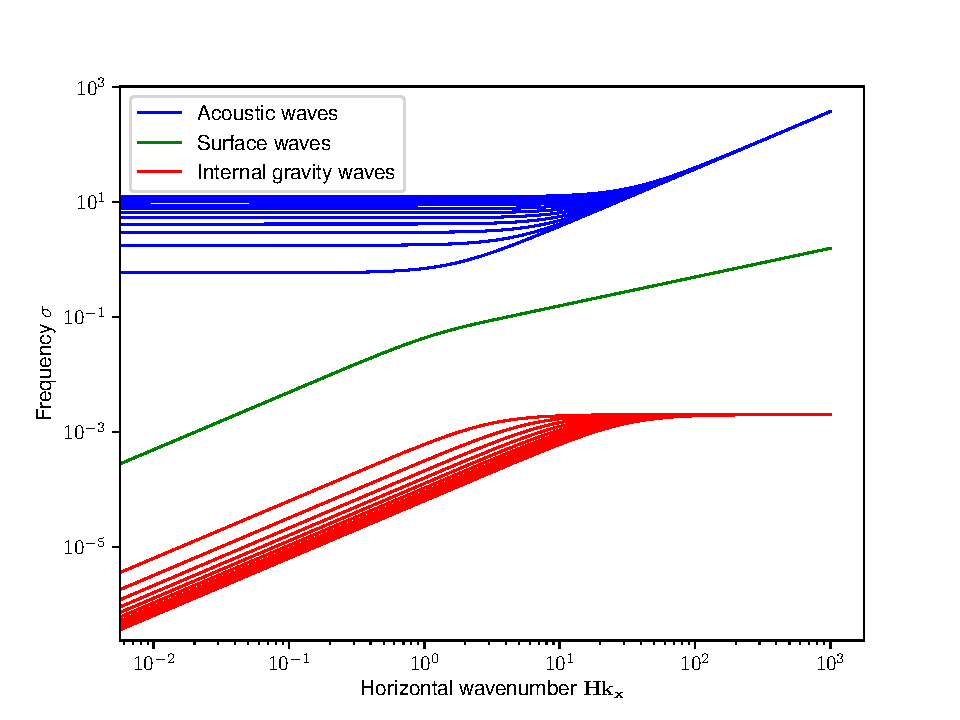
\includegraphics[width=15cm]{FIGURES/frequency}
}
\caption{Theoretical frequency $\sigma$ for internal gravity waves (modes 1 to 10), acoustic waves (modes 0 to 10) and for surface waves.}
\end{figure}
\begin{figure}[h]
\centerline{
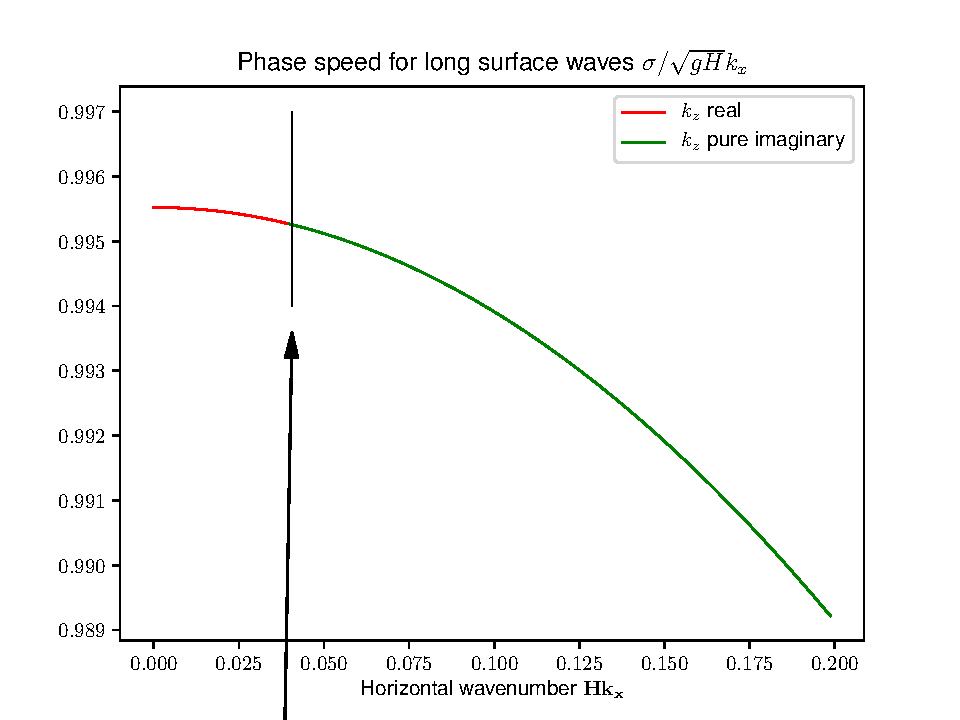
\includegraphics[width=15cm]{FIGURES/surfacewaves}
}
\caption{Numerical computed normalized frequency $\displaystyle \frac{\sigma}{\sqrt{gH}k_x}$ for long waves.}
\end{figure}
\begin{figure}[h]
\centerline{
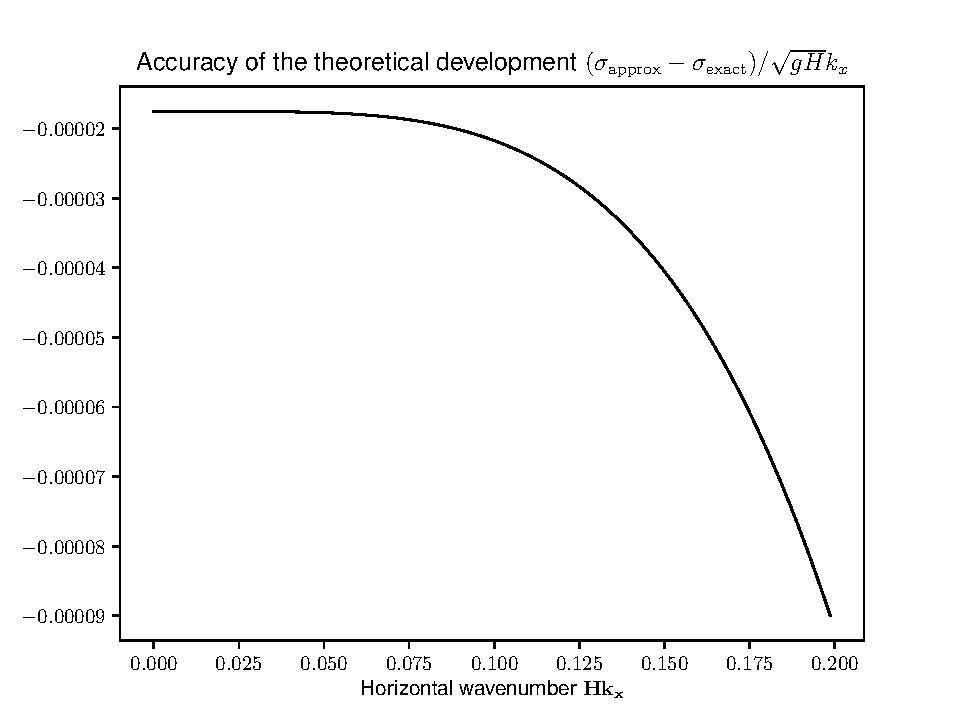
\includegraphics[width=15cm]{FIGURES/accuracy_longwaves}
}
\caption{Accuracy of the theoretical development: .}
\end{figure}